% An example second appendix from the example thesis thesis.tex.
\chapter{SUPPLEMENTARY MATERIALS FOR CHAPTER 3}

The material in this document supplement the information presented in Chapter \ref{ch:metrics}. Section \ref{sec:nbin} presents the procedure describing the selection of the number of bins.  

%\section*{Appendix}

\section{Selection of the Number of Bins} \label{sec:nbin}

Binned distance works for any type of data and for any null generating mechanism. It does not take into account the graphical elements in the plot, and the raw data is used. Binned distance can be used in situations where no distance measure is known for the particular plot type and hence it can be regarded as universal. But the choice of number of bins or the bin size highly affects the distance. A wrong choice may produce erroneous or conflicting results. Hence the choice of the number of bins is important.

The choice of number of bins or bin sizes is investigated with different types of data. Different null generating mechanisms are also used for the same data type. Null datasets are obtained for a true data using a null generating mechanism and hence a lineup is constructed. Mean binned distance is calculated between the true data and the null datasets and also among the null datasets. The number of bins for the binned distance are varied from 2 to 10 on both $x$ and $y$ direction and $\delta_{\hbox{lineup}}$ is calculated for each combination. Table \ref{tbl:bin1} and Table \ref{tbl:bin2} shows the type of data, the observed plot, the null generating mechanism, a typical null plot, the difference $\delta_{\hbox{lineup}}$ and also the maximum value of $\delta_{\hbox{lineup}}$, the $x$-bin and $y$-bin for which the maximum was obtained. The minimum $\delta_{\hbox{lineup}}$ is also reported to get an idea of the range of values.

%\begin{figure*}[hbtp]
%\centering
%\subfigure[]{
%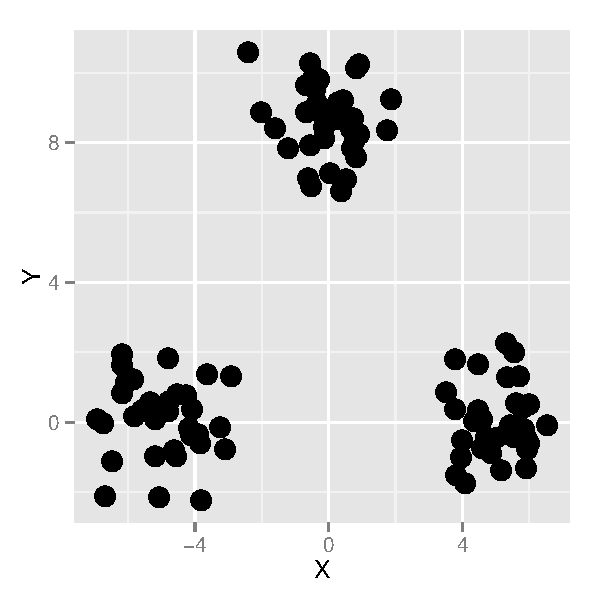
\includegraphics[scale=0.55]{data1.pdf}
%\label{nbin1_a}
%}
%\subfigure[]{
%\includegraphics[scale=0.55]{data1-nbin.pdf}
%\label{nbin1_b}
%}
%\label{nbin1}
%	\vspace{-.1in}
%\caption[Optional caption for list of figures]{(a) Plot showing the observed data (b) Binned distance plotted against the number of bins. }
%%{Caption of subfigures \subref{fig:subfig1}, \subref{fig:subfig2} and \subref{fig:subfig3}}
%\end{figure*}
%
%\begin{figure*}[hbtp]
%\centering
%\subfigure[]{
%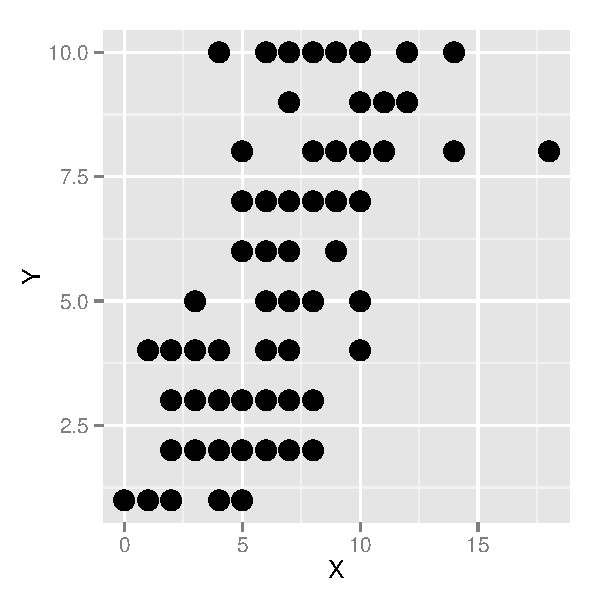
\includegraphics[scale=0.55]{data2.pdf}
%\label{nbin2_a}
%}
%\subfigure[]{
%\includegraphics[scale=0.55]{data2-nbin.pdf}
%\label{nbin2_b}
%}
%\label{nbin2}
%	\vspace{-.1in}
%\caption[Optional caption for list of figures]{(a) Plot showing the observed data (b) Binned distance plotted against the number of bins. }
%%{Caption of subfigures \subref{fig:subfig1}, \subref{fig:subfig2} and \subref{fig:subfig3}}
%\end{figure*}
%
%\begin{figure*}[hbtp]
%\centering
%\subfigure[]{
%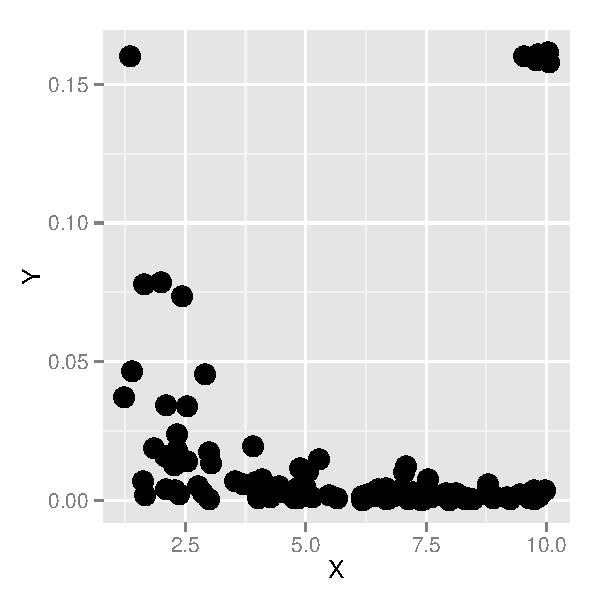
\includegraphics[scale=0.55]{data3.pdf}
%\label{nbin3_a}
%}
%\subfigure[]{
%\includegraphics[scale=0.55]{data3-nbin.pdf}
%\label{nbin3_b}
%}
%\label{nbin3}
%	\vspace{-.1in}
%\caption[Optional caption for list of figures]{(a) Plot showing the observed data (b) Binned distance plotted against the number of bins. }
%%{Caption of subfigures \subref{fig:subfig1}, \subref{fig:subfig2} and \subref{fig:subfig3}}
%\end{figure*}

\begin{table*}[hbtp]
\caption{Preferable number of bins for different types of observed data to calculate the binned distance.}
\vspace{0.1cm}
\centering 
\begin{tabular}{p{1.5cm}l c  p{1.6cm} c cc l c p{3.5cm}} 
\hline
 Type of Data & Observed Plot && Null Generating Mechanism & A typical null plot && & Difference && \hspace{0.5cm}(p, q, Max; Min) \\ %[0.5ex] % inserts table %heading 
%\hline
% Linear association & \begin{minipage}[h]{1.5cm} \begin{center} \scalebox{0.25}{\includegraphics{bin-select-data1.pdf}} \end{center} \end{minipage} && Permutation &  \begin{minipage}[h]{1.5cm} \begin{center} \scalebox{0.25}{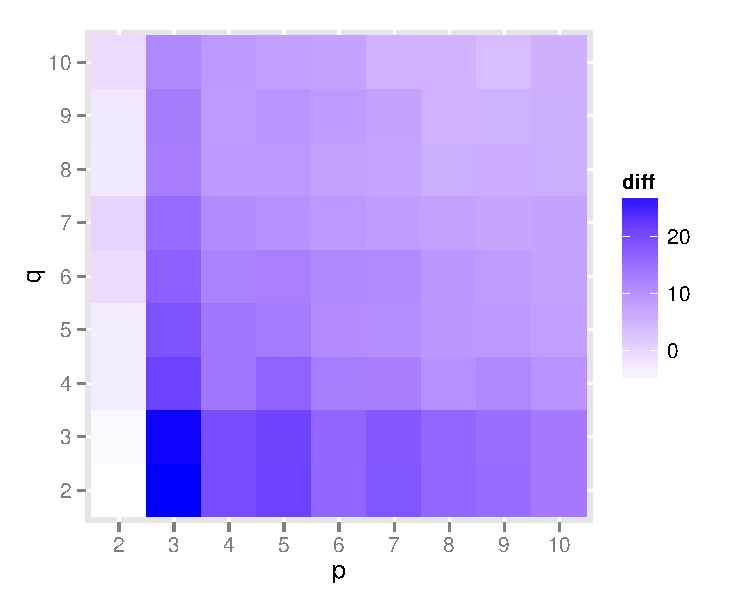
\includegraphics{bin-select-plot1.pdf}} \end{center} \end{minipage} &  \begin{minipage}[h]{1.5cm} \begin{center} \scalebox{0.25}{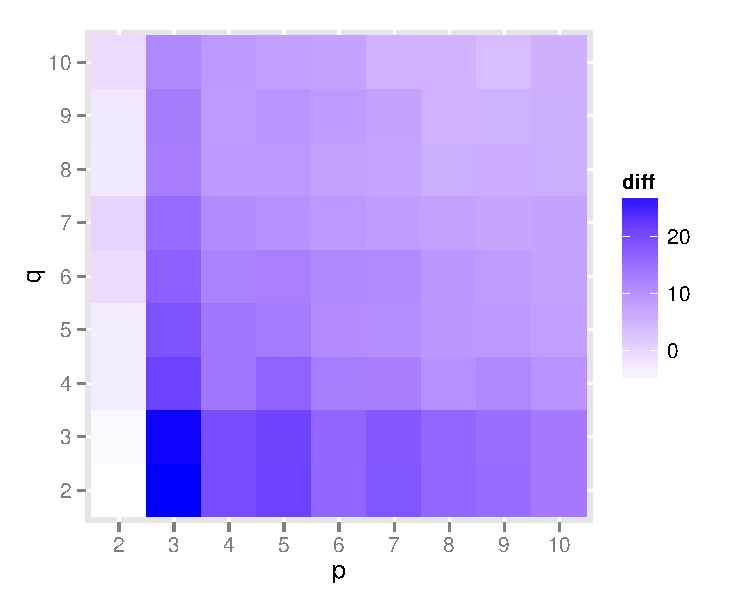
\includegraphics{bin-select-plot1.pdf}} \end{center} \end{minipage} &&           \hspace{0.8cm} small\\
 \hline
 Linear association & \begin{minipage}[h]{1.5cm} \begin{center} \scalebox{0.25}{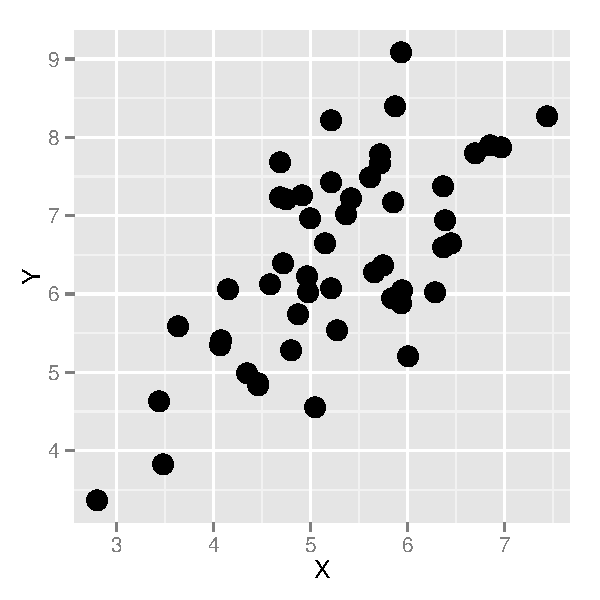
\includegraphics{anscombe-1.pdf}} \end{center} \end{minipage} && Permutation &  \begin{minipage}[h]{1.5cm} \begin{center} \scalebox{0.25}{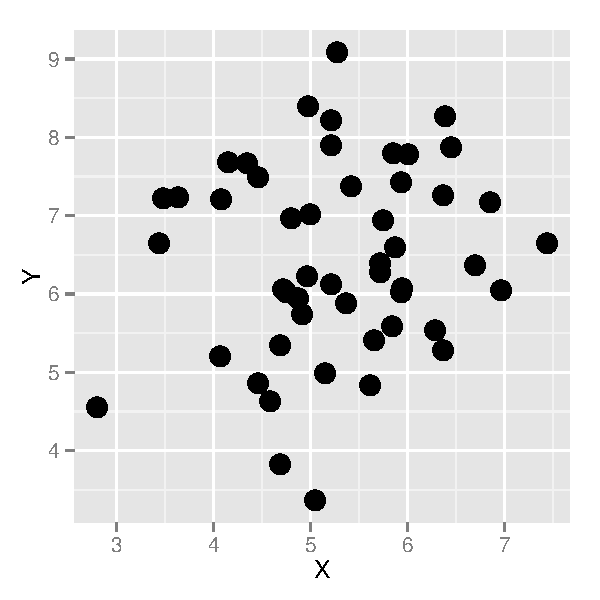
\includegraphics{anscombe-null-1.pdf}} \end{center} \end{minipage} &&&  \begin{minipage}[h]{1.5cm} \begin{center} \scalebox{0.25}{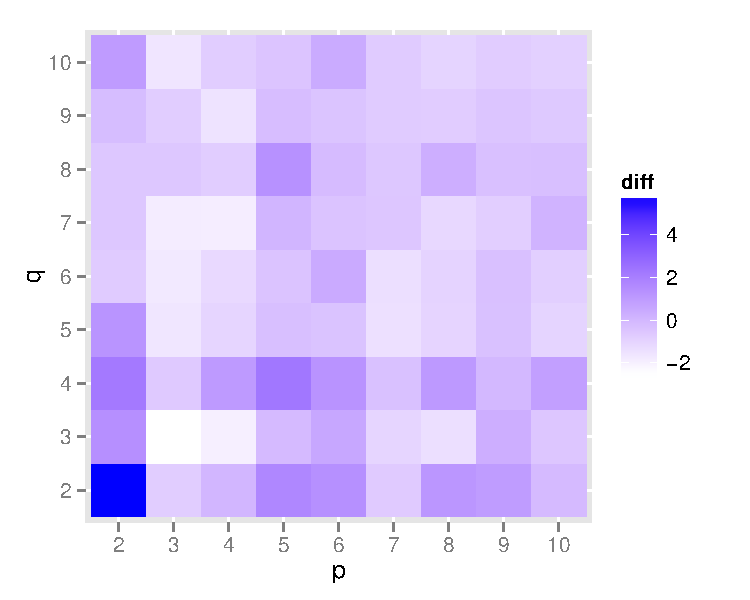
\includegraphics{anscombe-nbin-1.pdf}} \end{center} \end{minipage} &&           \hspace{0.8cm} (2, 2, 5.7 ; - 2.5)\\
 \hline
Nonlinear relationship & \begin{minipage}[h]{1.5cm} \begin{center} \scalebox{0.25}{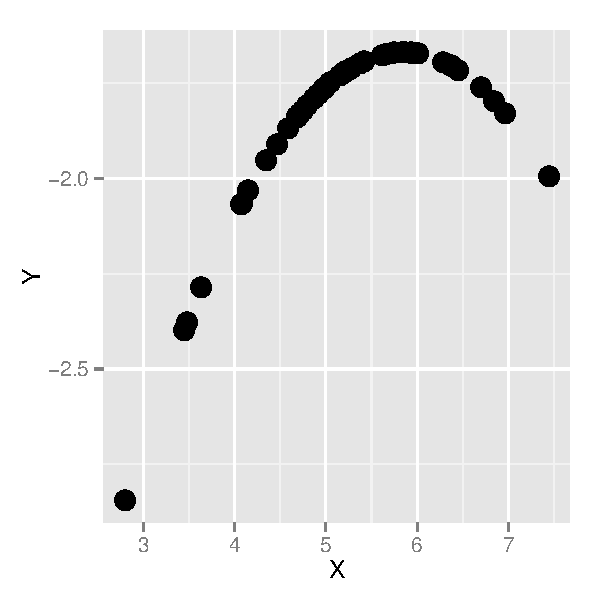
\includegraphics{anscombe-2.pdf}} \end{center} \end{minipage} && Permutation &  \begin{minipage}[h]{1.5cm} \begin{center} \scalebox{0.25}{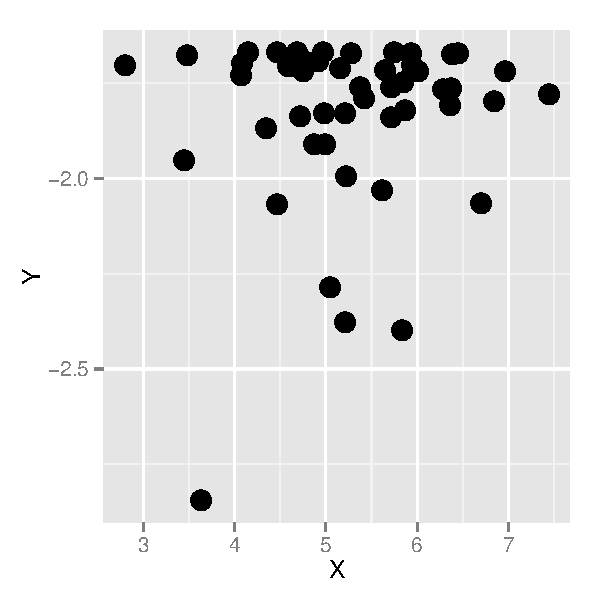
\includegraphics{anscombe-null-2.pdf}} \end{center} \end{minipage} &&&  \begin{minipage}[h]{1.5cm} \begin{center} \scalebox{0.25}{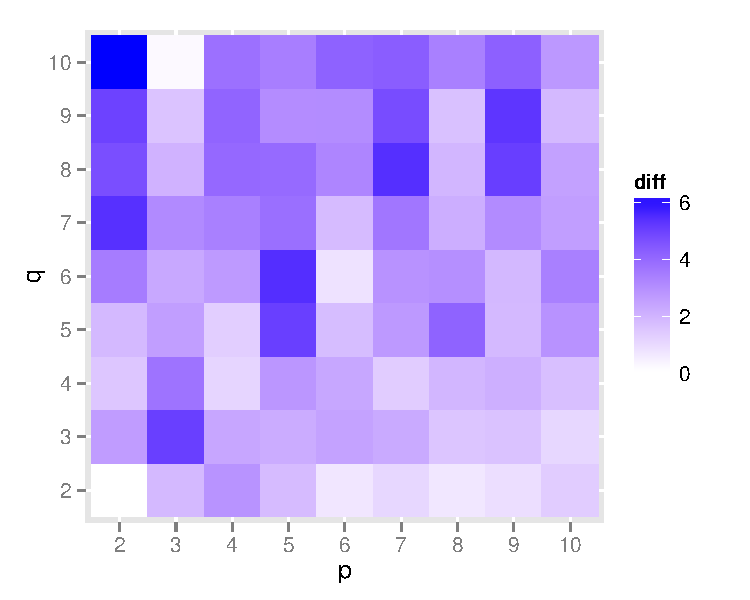
\includegraphics{anscombe-nbin-2.pdf}} \end{center} \end{minipage} &&           \hspace{0.6cm} (2, 10, 6.2 ; - 0.0)\\
 \hline
 Linear relation with outliers & \begin{minipage}[h]{1.5cm} \begin{center} \scalebox{0.25}{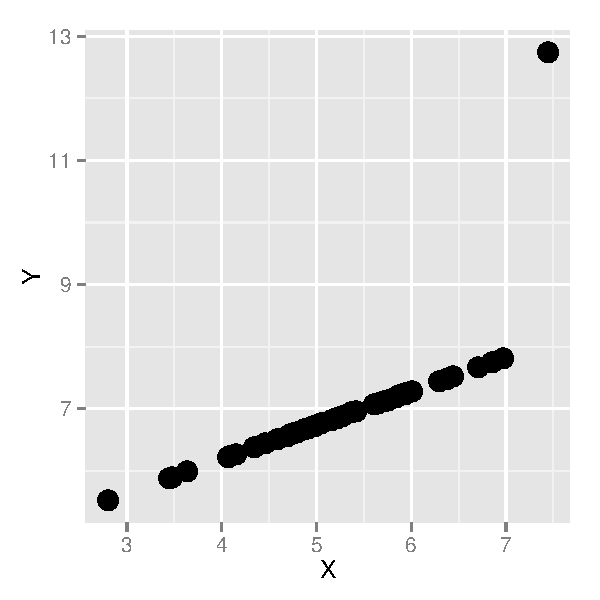
\includegraphics{anscombe-3.pdf}} \end{center} \end{minipage} && Permutation &  \begin{minipage}[h]{1.5cm} \begin{center} \scalebox{0.25}{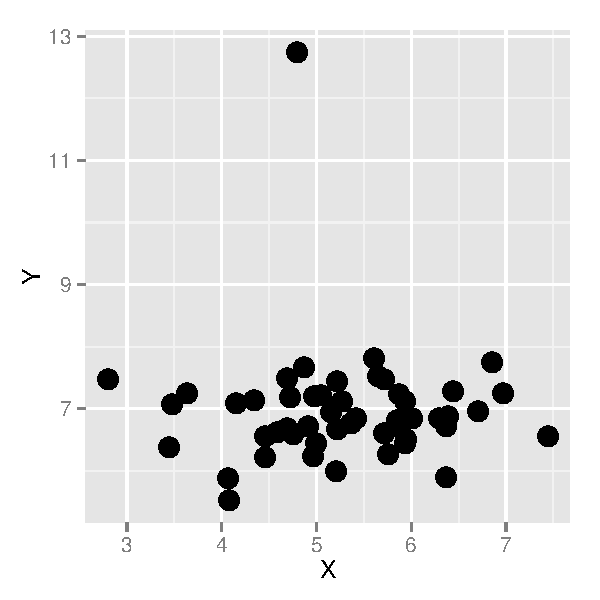
\includegraphics{anscombe-null-3.pdf}} \end{center} \end{minipage} &&&  \begin{minipage}[h]{1.5cm} \begin{center} \scalebox{0.25}{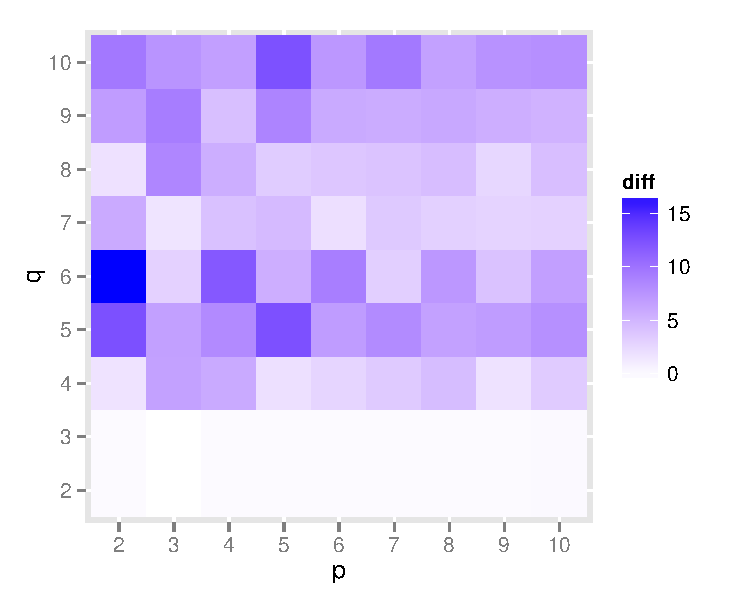
\includegraphics{anscombe-nbin-3.pdf}} \end{center} \end{minipage} &&           \hspace{0.6cm} (2, 6, 16.7 ; - 0.4)\\
 \hline
 Same values with one outlier & \begin{minipage}[h]{1.5cm} \begin{center} \scalebox{0.25}{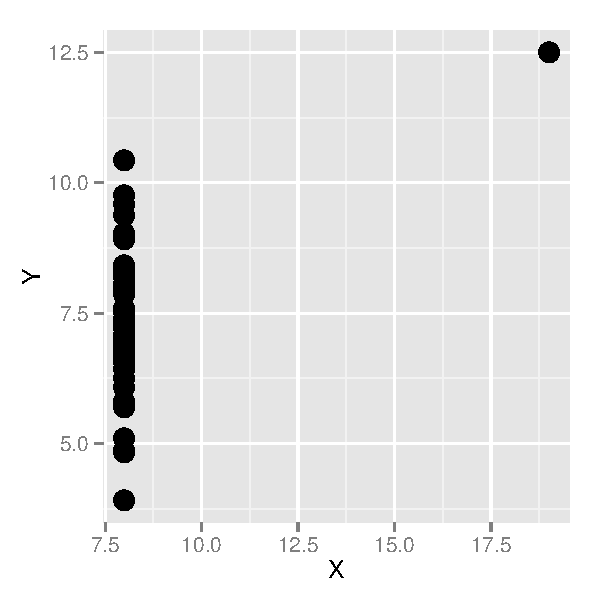
\includegraphics{anscombe-4.pdf}} \end{center} \end{minipage} && Simulation from a \emph{Poi(9)} distribution &  \begin{minipage}[h]{1.5cm} \begin{center} \scalebox{0.25}{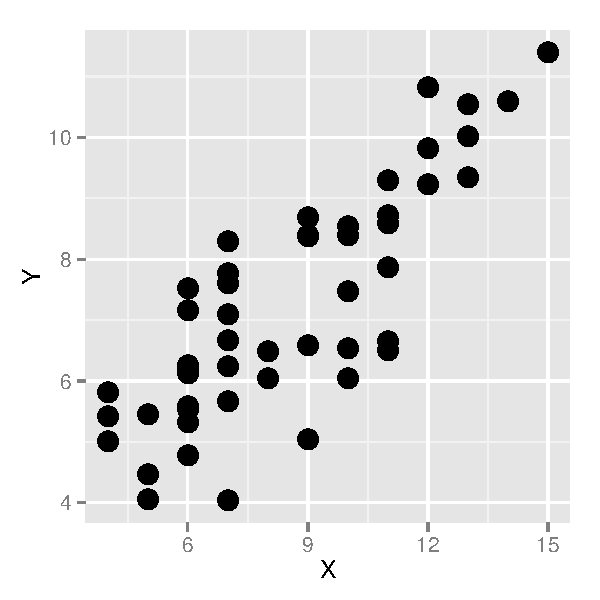
\includegraphics{anscombe-null-4.pdf}} \end{center} \end{minipage} &&&  \begin{minipage}[h]{1.5cm} \begin{center} \scalebox{0.25}{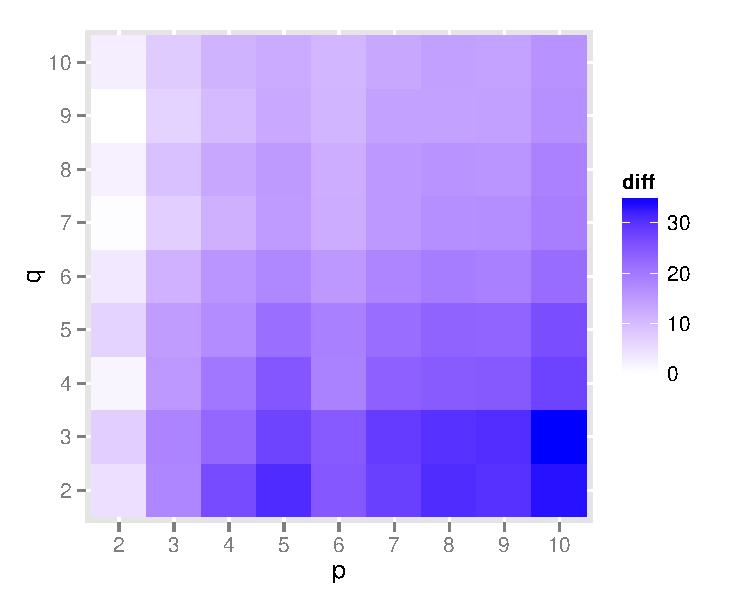
\includegraphics{anscombe-nbin-4.pdf}} \end{center} \end{minipage} &&           \hspace{0.5cm}(10, 3, 34.3 ; - 0.1)\\
 \hline
    Clusters & \begin{minipage}[h]{1.5cm} \begin{center} \scalebox{0.25}{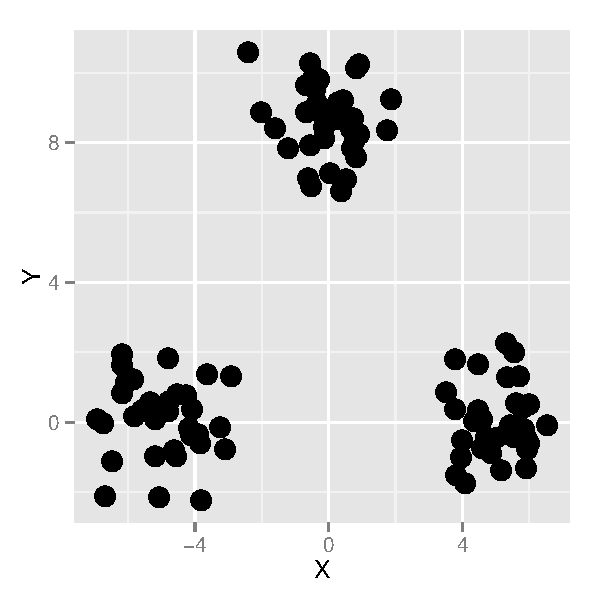
\includegraphics{data1.pdf}} \end{center} \end{minipage} && Permutation &  \begin{minipage}[h]{1.5cm} \begin{center} \scalebox{0.25}{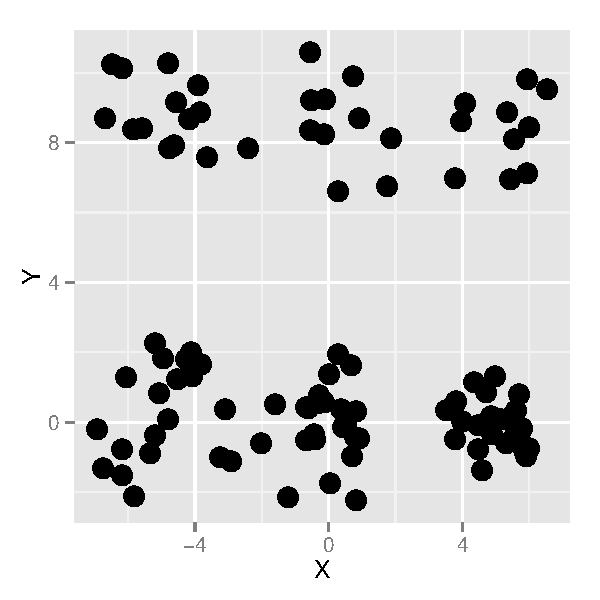
\includegraphics{null1.pdf}} \end{center} \end{minipage} &&&  \begin{minipage}[h]{1.5cm} \begin{center} \scalebox{0.25}{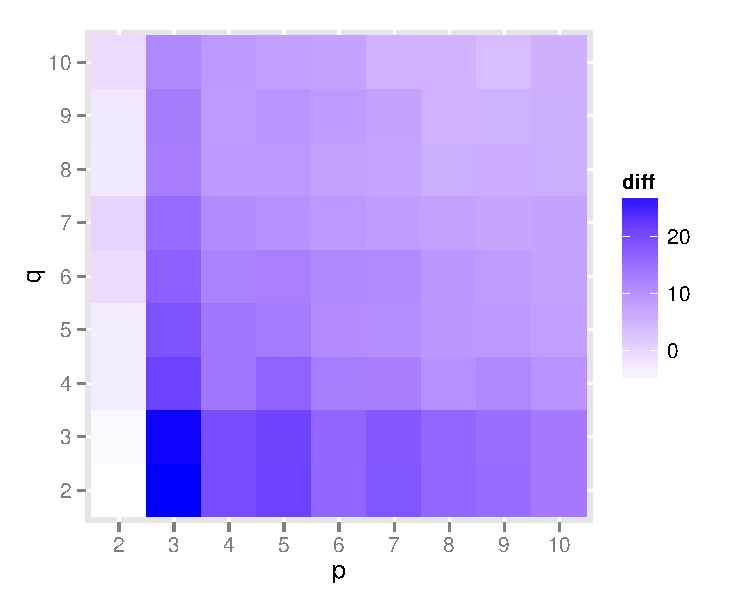
\includegraphics{bin-select-plot1.pdf}} \end{center} \end{minipage} &&           \hspace{0.6cm} (3, 2, 27.6 ; - 5.7)\\
 \hline
 Categorical & \begin{minipage}[h]{1.5cm} \begin{center} \scalebox{0.25}{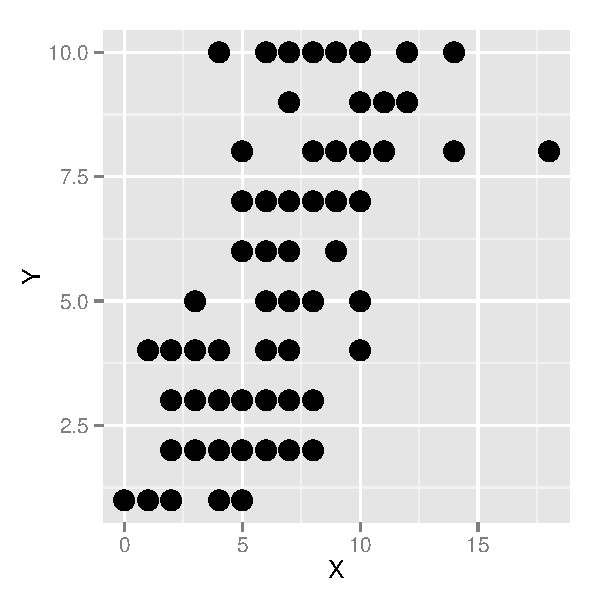
\includegraphics{data2.pdf}} \end{center} \end{minipage} && Simulation from a Normal distribution &  \begin{minipage}[h]{1.5cm} \begin{center} \scalebox{0.25}{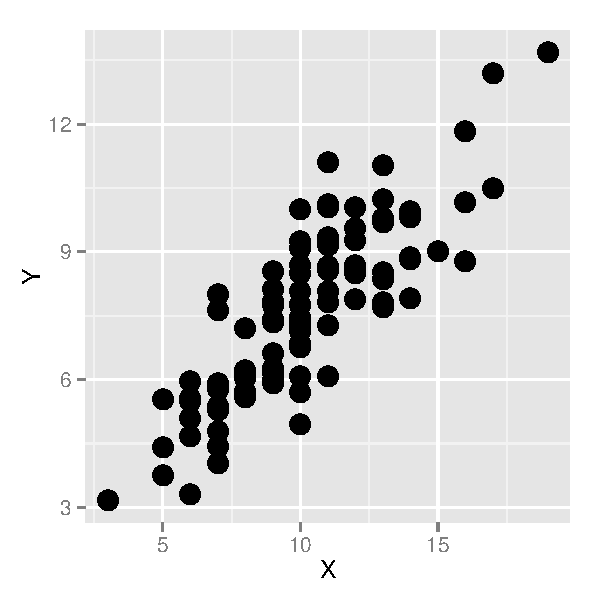
\includegraphics{null2.pdf}} \end{center} \end{minipage} &&&  \begin{minipage}[h]{1.5cm} \begin{center} \scalebox{0.25}{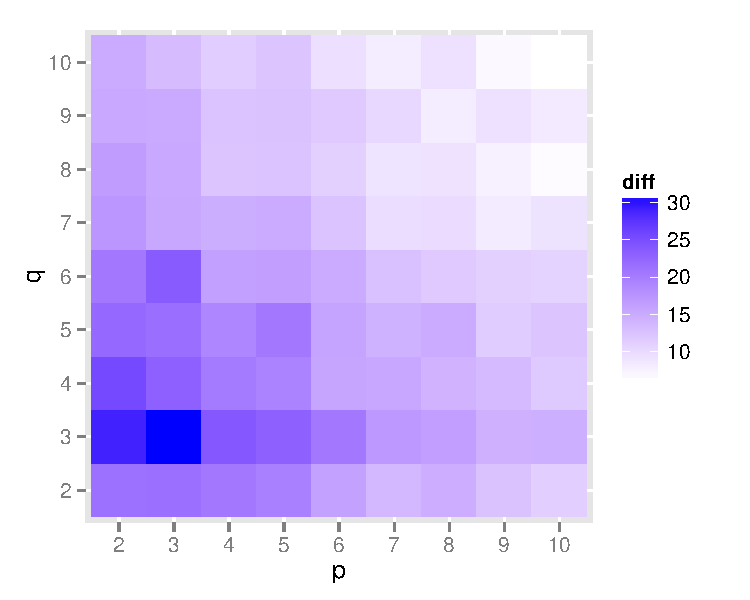
\includegraphics{bin-select-plot2.pdf}} \end{center} \end{minipage} &&           \hspace{0.8cm} (3, 3, 30.7; 6.2) \\
 \hline
%Clusters & \begin{minipage}[h]{1.5cm} \begin{center} \scalebox{0.25}{\includegraphics{bin-select-data2.pdf}} \end{center} \end{minipage} && Permutation &  \begin{minipage}[h]{1.5cm} \begin{center} \scalebox{0.25}{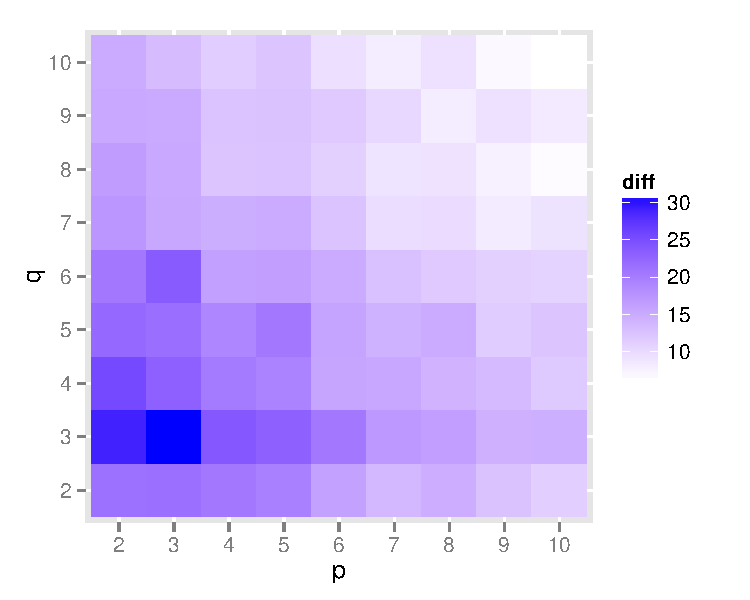
\includegraphics{bin-select-plot2.pdf}} \end{center} \end{minipage} && \hspace{0.8cm} small\\
% \hline
% Discrete vs. Continuous & \begin{minipage}[h]{1.5cm} \begin{center} \scalebox{0.25}{\includegraphics{bin-select-data3.pdf}} \end{center} \end{minipage} && Simulation from a specific distribution &  \begin{minipage}[h]{1.5cm} \begin{center} \scalebox{0.25}{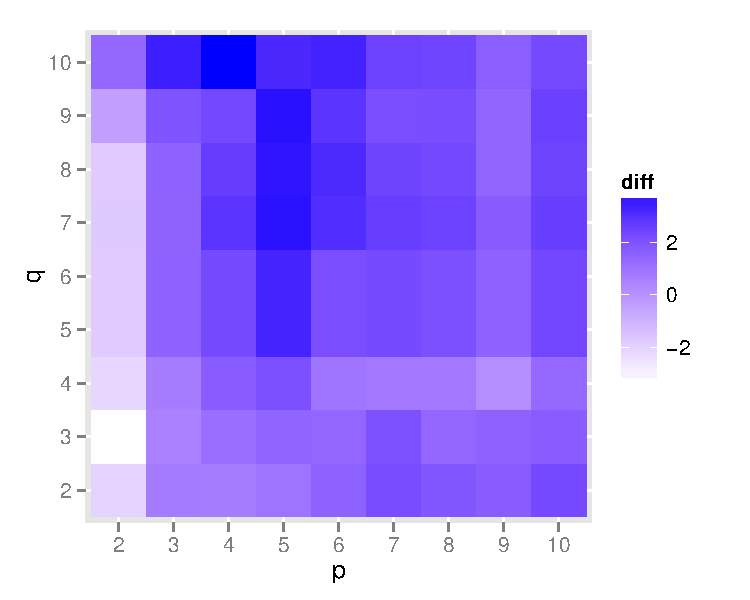
\includegraphics{bin-select-plot3.pdf}} \end{center} \end{minipage} && \hspace{0.8cm} small\\
% \hline
% Discrete vs. Continuous & \begin{minipage}[h]{1.5cm} \begin{center} \scalebox{0.25}{\includegraphics{bin-select-data4.pdf}} \end{center} \end{minipage} && Permutation &  \begin{minipage}[h]{1.5cm} \begin{center} \scalebox{0.25}{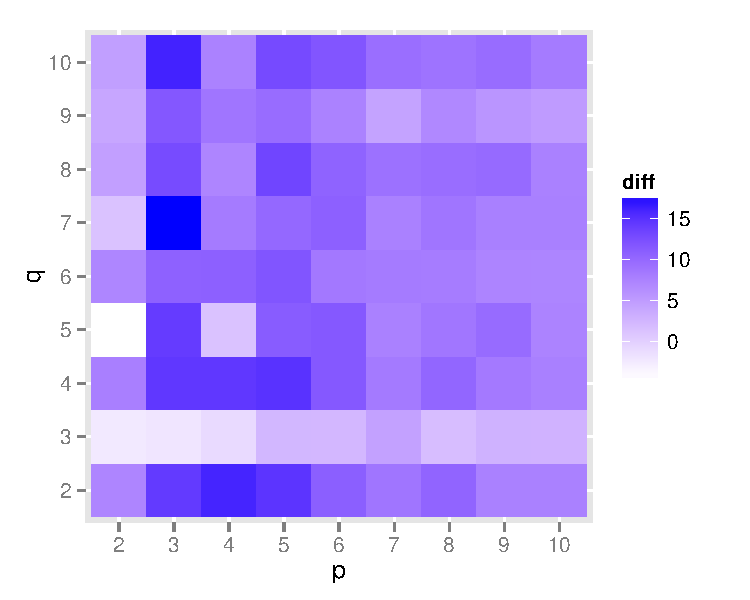
\includegraphics{bin-select-plot4.pdf}} \end{center} \end{minipage} && \hspace{0.8cm} large\\
% \hline
%Presence of Outlier(s) & \begin{minipage}[h]{1.5cm} \begin{center} \scalebox{0.25}{\includegraphics{bin-select-data5.pdf}} \end{center} \end{minipage} && Simulation from a specific distribution &  \begin{minipage}[h]{1.5cm} \begin{center} \scalebox{0.25}{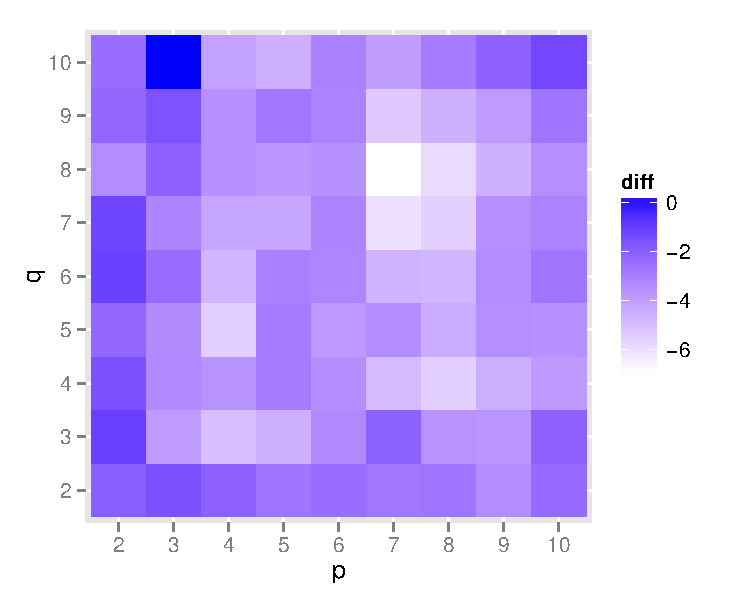
\includegraphics{bin-select-plot5.pdf}} \end{center} \end{minipage} && \hspace{0.8cm} small\\
% \hline
\end{tabular}
\label{tbl:bin1}
\end{table*}

%\newpage
\begin{table*}[hbtp]
\caption{Preferable number of bins for different types of observed data to calculate the binned distance.}
\vspace{0.1cm}
\centering 
\begin{tabular}{p{1.5cm}l c  p{1.6cm} c cc l c p{3.5cm}} 
\hline
 Type of Data & Observed Plot && Null Generating Mechanism & A typical null plot && & Difference &&  \hspace{0.5cm}(p, q, Max; Min) \\ %[0.5ex] % inserts table %heading 
 \hline
Nonlinear relation with outliers & \begin{minipage}[h]{1.5cm} \begin{center} \scalebox{0.25}{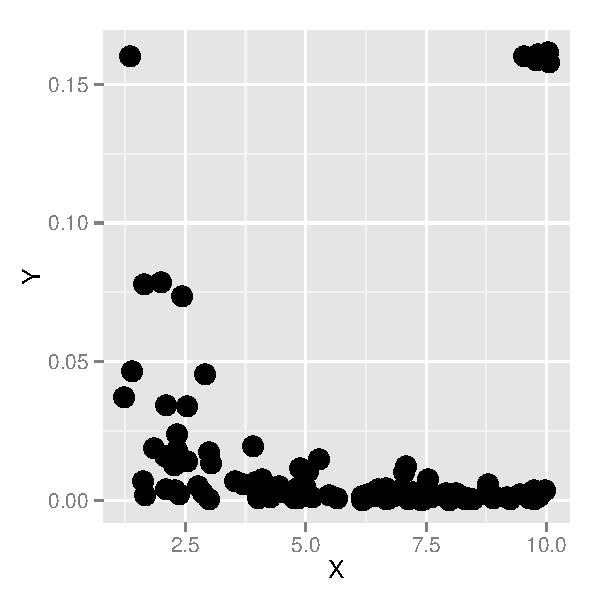
\includegraphics{data3.pdf}} \end{center} \end{minipage} && Permutation &  \begin{minipage}[h]{1.5cm} \begin{center} \scalebox{0.25}{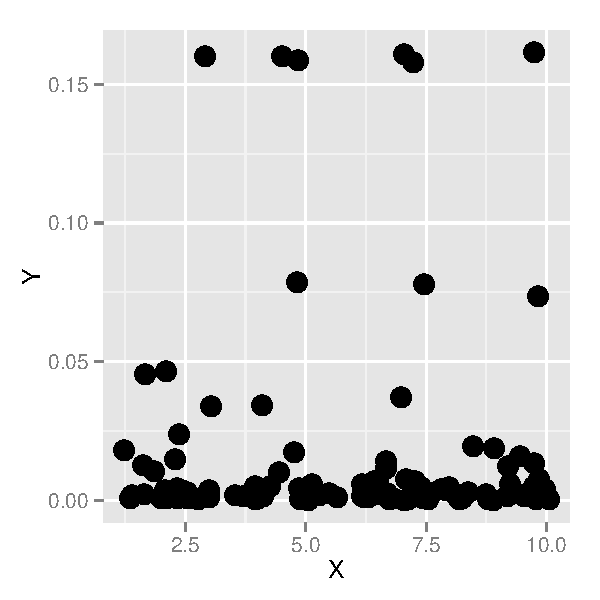
\includegraphics{null3.pdf}} \end{center} \end{minipage} &&&  \begin{minipage}[h]{1.5cm} \begin{center} \scalebox{0.25}{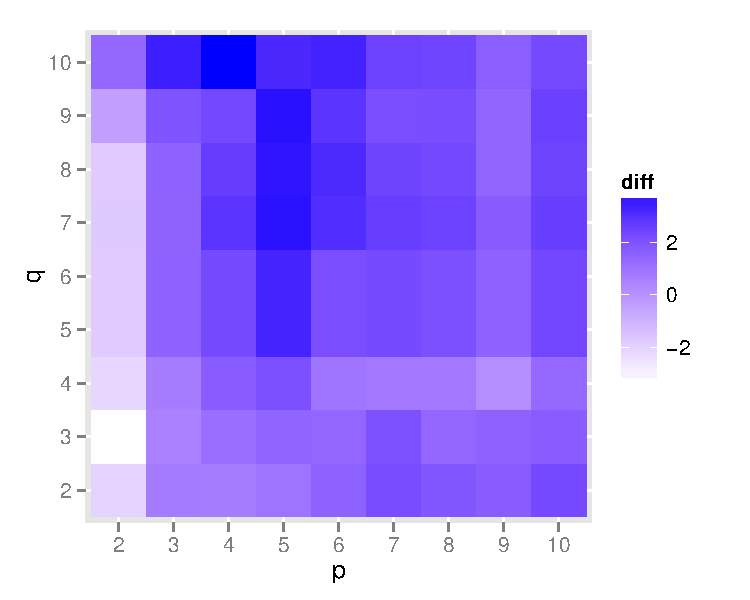
\includegraphics{bin-select-plot3.pdf}} \end{center} \end{minipage} &&           \hspace{0.8cm} (4, 10, 3.9; -3.4) \\
 \hline
Linear relationship with outlier  & \begin{minipage}[h]{1.5cm} \begin{center} \scalebox{0.25}{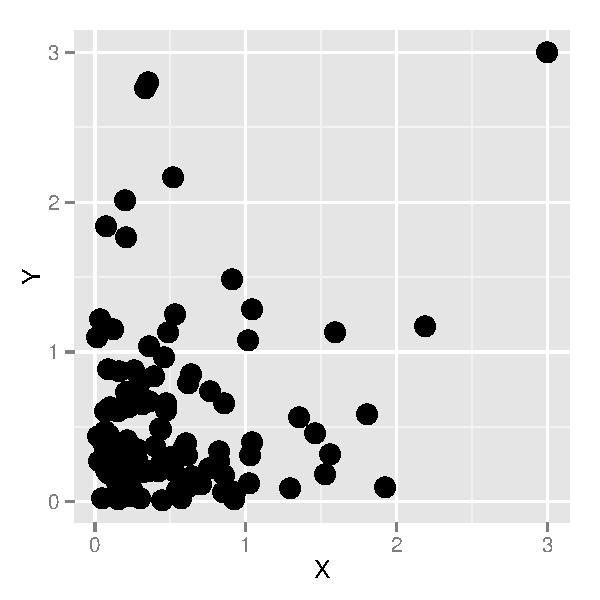
\includegraphics{data5.pdf}} \end{center} \end{minipage} && Permutation &  \begin{minipage}[h]{1.5cm} \begin{center} \scalebox{0.25}{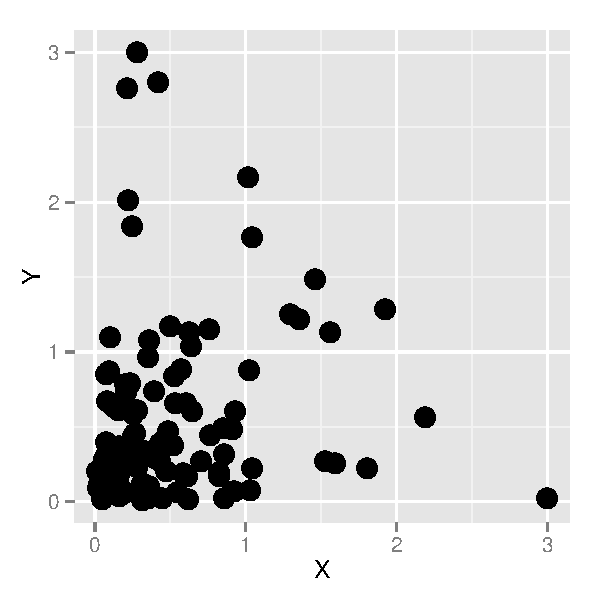
\includegraphics{null5.pdf}} \end{center} \end{minipage} &&&  \begin{minipage}[h]{1.5cm} \begin{center} \scalebox{0.25}{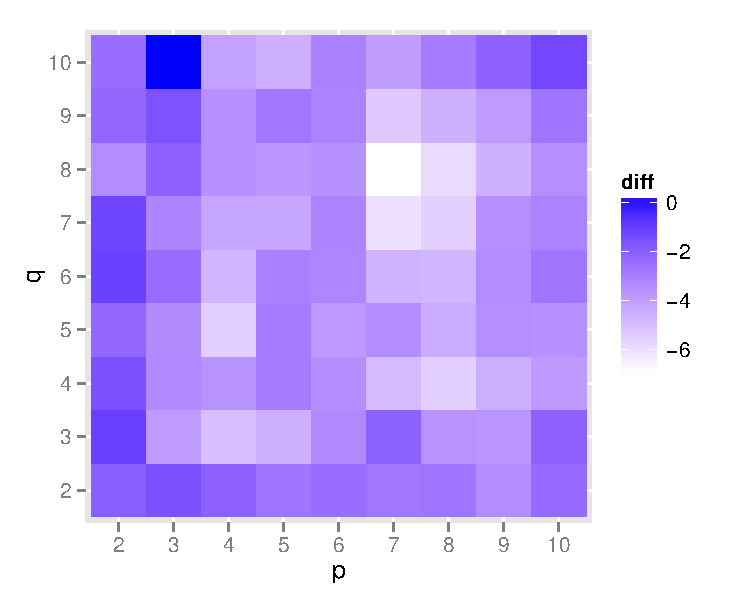
\includegraphics{bin-select-plot5.pdf}} \end{center} \end{minipage} &&           \hspace{0.8cm} (3, 10, 0.3; -7.1) \\
 \hline
 Residual Plot & \begin{minipage}[h]{1.5cm} \begin{center} \scalebox{0.25}{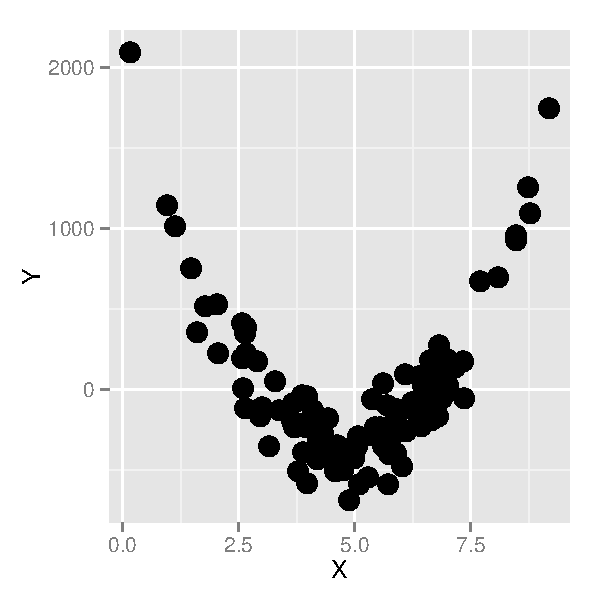
\includegraphics{data4.pdf}} \end{center} \end{minipage} && Simulation from the null model &  \begin{minipage}[h]{1.5cm} \begin{center} \scalebox{0.25}{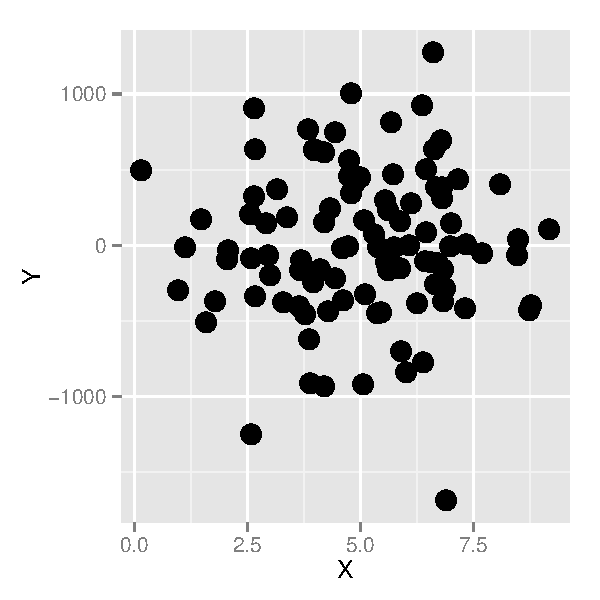
\includegraphics{null4.pdf}} \end{center} \end{minipage} &&&  \begin{minipage}[h]{1.5cm} \begin{center} \scalebox{0.25}{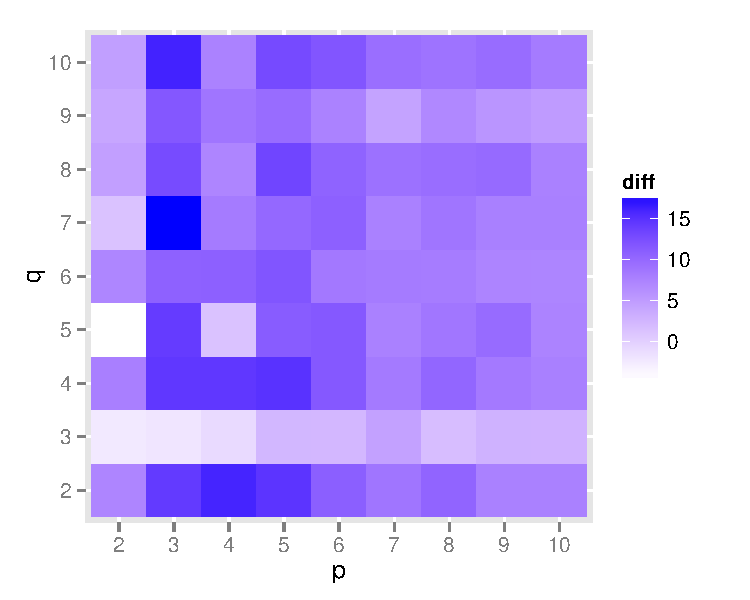
\includegraphics{bin-select-plot4.pdf}} \end{center} \end{minipage} &&           \hspace{0.8cm} (3, 7, 17.8; -4.5)\\
 \hline
 Residual Plot & \begin{minipage}[h]{1.5cm} \begin{center} \scalebox{0.25}{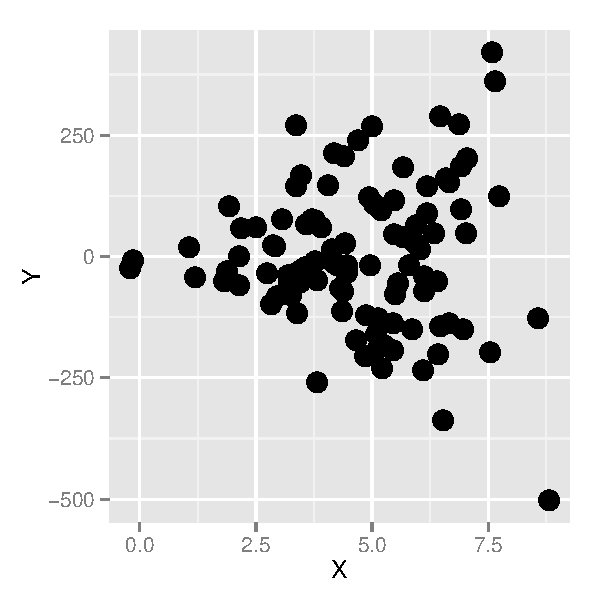
\includegraphics{data6.pdf}} \end{center} \end{minipage} && Simulation from the null model &  \begin{minipage}[h]{1.5cm} \begin{center} \scalebox{0.25}{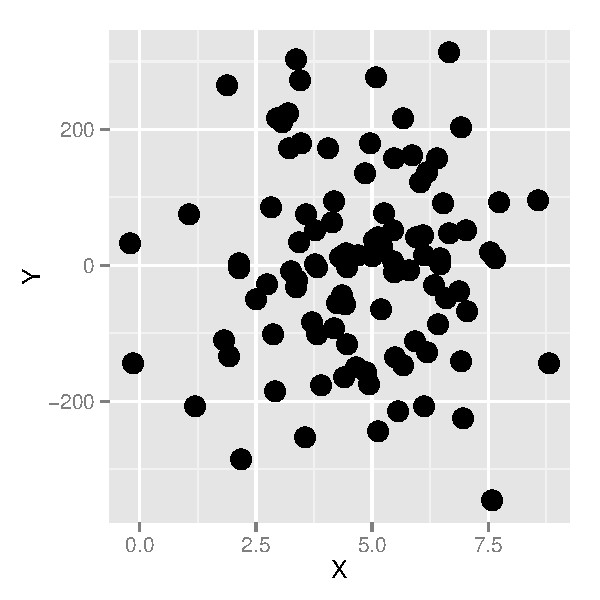
\includegraphics{null6.pdf}} \end{center} \end{minipage} &&&  \begin{minipage}[h]{1.5cm} \begin{center} \scalebox{0.25}{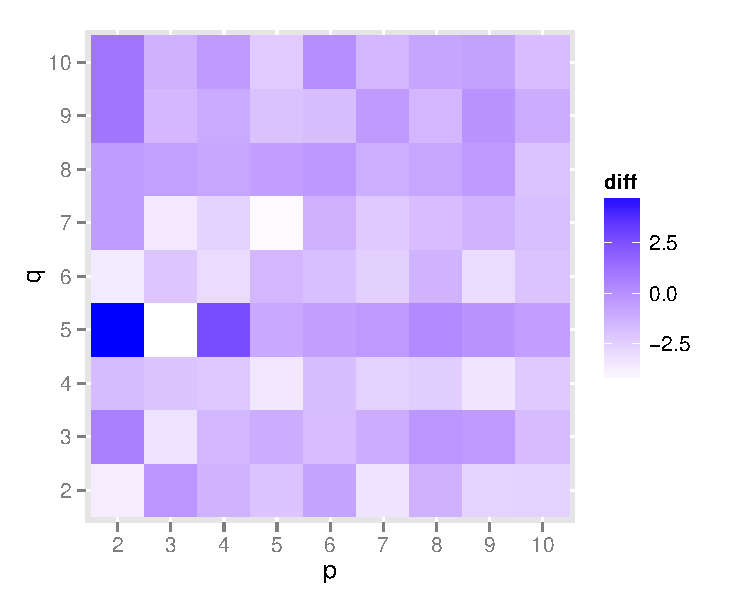
\includegraphics{bin-select-plot6.pdf}} \end{center} \end{minipage} &&           \hspace{0.8cm} (2, 5, 4.8; -4.4)\\
 \hline
Spiral data & \begin{minipage}[h]{1.5cm} \begin{center} \scalebox{0.25}{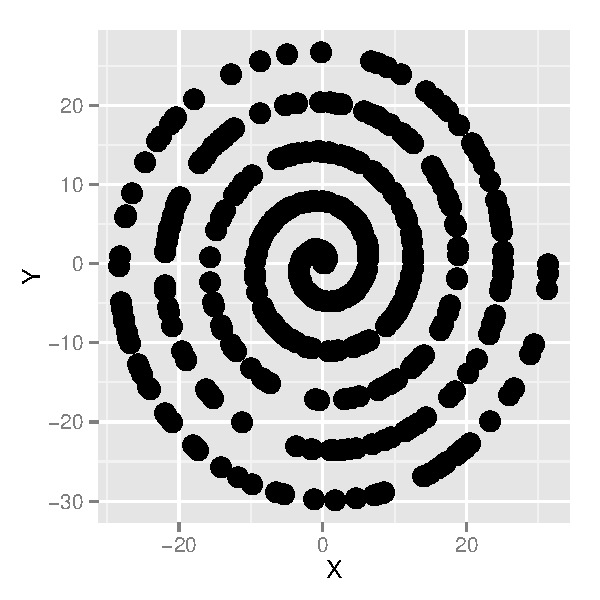
\includegraphics{data7.pdf}} \end{center} \end{minipage} && Permutation &  \begin{minipage}[h]{1.5cm} \begin{center} \scalebox{0.25}{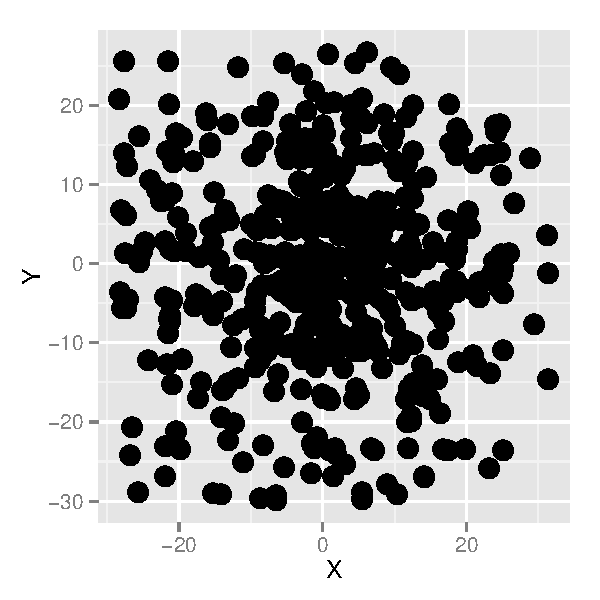
\includegraphics{null7.pdf}} \end{center} \end{minipage} &&&  \begin{minipage}[h]{1.5cm} \begin{center} \scalebox{0.25}{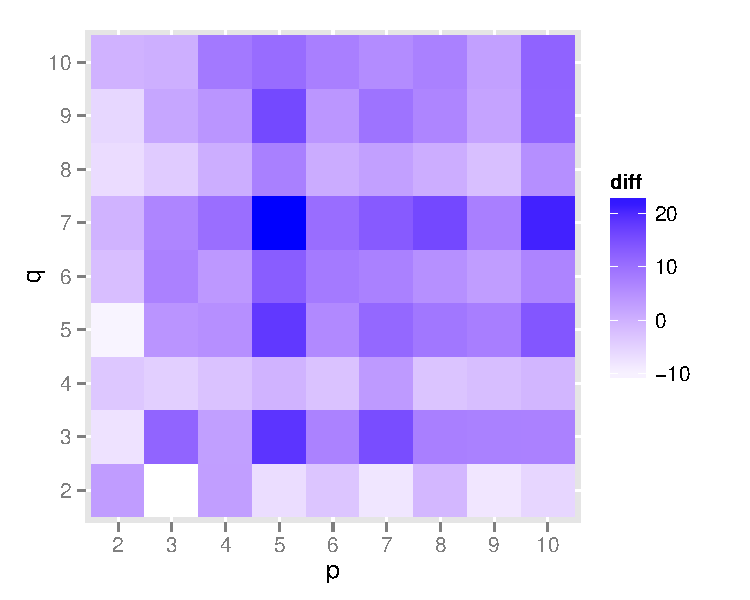
\includegraphics{bin-select-plot7.pdf}} \end{center} \end{minipage} &&           \hspace{0.6cm} (5, 7, 23.6; -11.9)\\
 \hline
Contaminated data & \begin{minipage}[h]{1.5cm} \begin{center} \scalebox{0.25}{\includegraphics{data8.pdf}} \end{center} \end{minipage} && Permutation &  \begin{minipage}[h]{1.5cm} \begin{center} \scalebox{0.25}{\includegraphics{null8.pdf}} \end{center} \end{minipage} &&&  \begin{minipage}[h]{1.5cm} \begin{center} \scalebox{0.25}{\includegraphics{bin-select-plot8.pdf}} \end{center} \end{minipage} &&           \hspace{0.8cm} (5, 3, 8.1; -2.5)\\
 \hline
%Clusters & \begin{minipage}[h]{1.5cm} \begin{center} \scalebox{0.25}{\includegraphics{bin-select-data2.pdf}} \end{center} \end{minipage} && Permutation &  \begin{minipage}[h]{1.5cm} \begin{center} \scalebox{0.25}{\includegraphics{bin-select-plot2.pdf}} \end{center} \end{minipage} && \hspace{0.8cm} small\\
% \hline
% Discrete vs. Continuous & \begin{minipage}[h]{1.5cm} \begin{center} \scalebox{0.25}{\includegraphics{bin-select-data3.pdf}} \end{center} \end{minipage} && Simulation from a specific distribution &  \begin{minipage}[h]{1.5cm} \begin{center} \scalebox{0.25}{\includegraphics{bin-select-plot3.pdf}} \end{center} \end{minipage} && \hspace{0.8cm} small\\
% \hline
% Discrete vs. Continuous & \begin{minipage}[h]{1.5cm} \begin{center} \scalebox{0.25}{\includegraphics{bin-select-data4.pdf}} \end{center} \end{minipage} && Permutation &  \begin{minipage}[h]{1.5cm} \begin{center} \scalebox{0.25}{\includegraphics{bin-select-plot4.pdf}} \end{center} \end{minipage} && \hspace{0.8cm} large\\
% \hline
%Presence of Outlier(s) & \begin{minipage}[h]{1.5cm} \begin{center} \scalebox{0.25}{\includegraphics{bin-select-data5.pdf}} \end{center} \end{minipage} && Simulation from a specific distribution &  \begin{minipage}[h]{1.5cm} \begin{center} \scalebox{0.25}{\includegraphics{bin-select-plot5.pdf}} \end{center} \end{minipage} && \hspace{0.8cm} small\\
% \hline
\end{tabular}
\label{tbl:bin2}
\end{table*}

The rationale behind selecting different types of data is to investigate how the optimal number of bins or bin sizes varies with different types of data. The different null generating mechanisms are also selected for the same reason. In Table \ref{tbl:bin1} the first four observed data plots corresponds to the datasets described by Francis Anscombe \citep{anscombe:1972} but with large number of data points. Although the datasets have the same pattern, the datasets do not follow the properties of Anscombe's quartet. The fifth dataset is a data with 3 distinct clusters. In Table \ref{tbl:bin2}, the first dataset shows a categorical data. The second and the third data are non-linear and linear association with the presence of outliers. The fourth and fifth datasets are the residual plots with curved pattern and non-constant variance pattern. The sixth data is a spiral data while the seventh one is a data with contamination. 

The differences, $\delta_{\hbox{lineup}}$, are represented in a tile plot where each tile gives the difference for each combination. The dark blue shows higher values while the white shows lower values. It can be seen that the plots look different for the different datasets. Hence the optimal number of bins varies from data to data. No specific pattern is evident in the plot. But overall it can be seen that for strong linear relationship, small number of bins should be preferred over large number of bins. Also when outlier is present in the data, larger number of bins is preferred at least in one axis.

It is important to mention at this point that Table \ref{tbl:bin1} and Table \ref{tbl:bin2} is not meant to provide any guidelines for the selection of number of bins. The Tables only show that the binned distance is highly affected by the number of bins and the type of data. It is advisable to find the optimal number of bins for a given data before using the binned distance.